
\section{Network Architecture}
\label{sec:arch}

%An in-depth examination of architectures via trial and error is left  future 

We begin with the notion that the discretization procedure outlined in Section \ref{sec:simulation} produces $25\times 25$ ``energy-scale'' images in one channel -- a High Energy Physics analogue of a grayscale image. We note that the images we work with are \emph{sparse} -- roughly 12\% of pixels are active on average. Future work can build on efficient techniques for exploiting the sparse nature of these images -- i.e., memoized convolutions. However, since speed is not our driving force in this work, we utilized convolution implementations defined for dense inputs.  We also studies fully connected MaxOut networks~\cite{maxout:goodfellow}.

\subsubsection{Architectural Selection} % (fold)
\label{ssub:architectural_selection}
For the MaxOut network, we utilize \textbf{N fully connected layers, of sizes (X,Y,Z), which each use the MaxOut activation.  These layers are followed by a fully connected logistic layer for classification.... NEED INFO AND CONFIRMATION FROM LUKE.}.  This network is trained (and evaluated) on un-normalized jet-images using the transverse energy for the pixel intensities

For the deep convolution networks, we utilize a simple convolutional architecture consisting of two sequential \texttt{[Conv + Max-Pool + Dropout]} units, followed by two fully connected, dense layers. A conceptual visualization of the network architecture can be seen in Figure~\ref{fig:arch}.
\begin{figure}[!htbp]
  \centering
  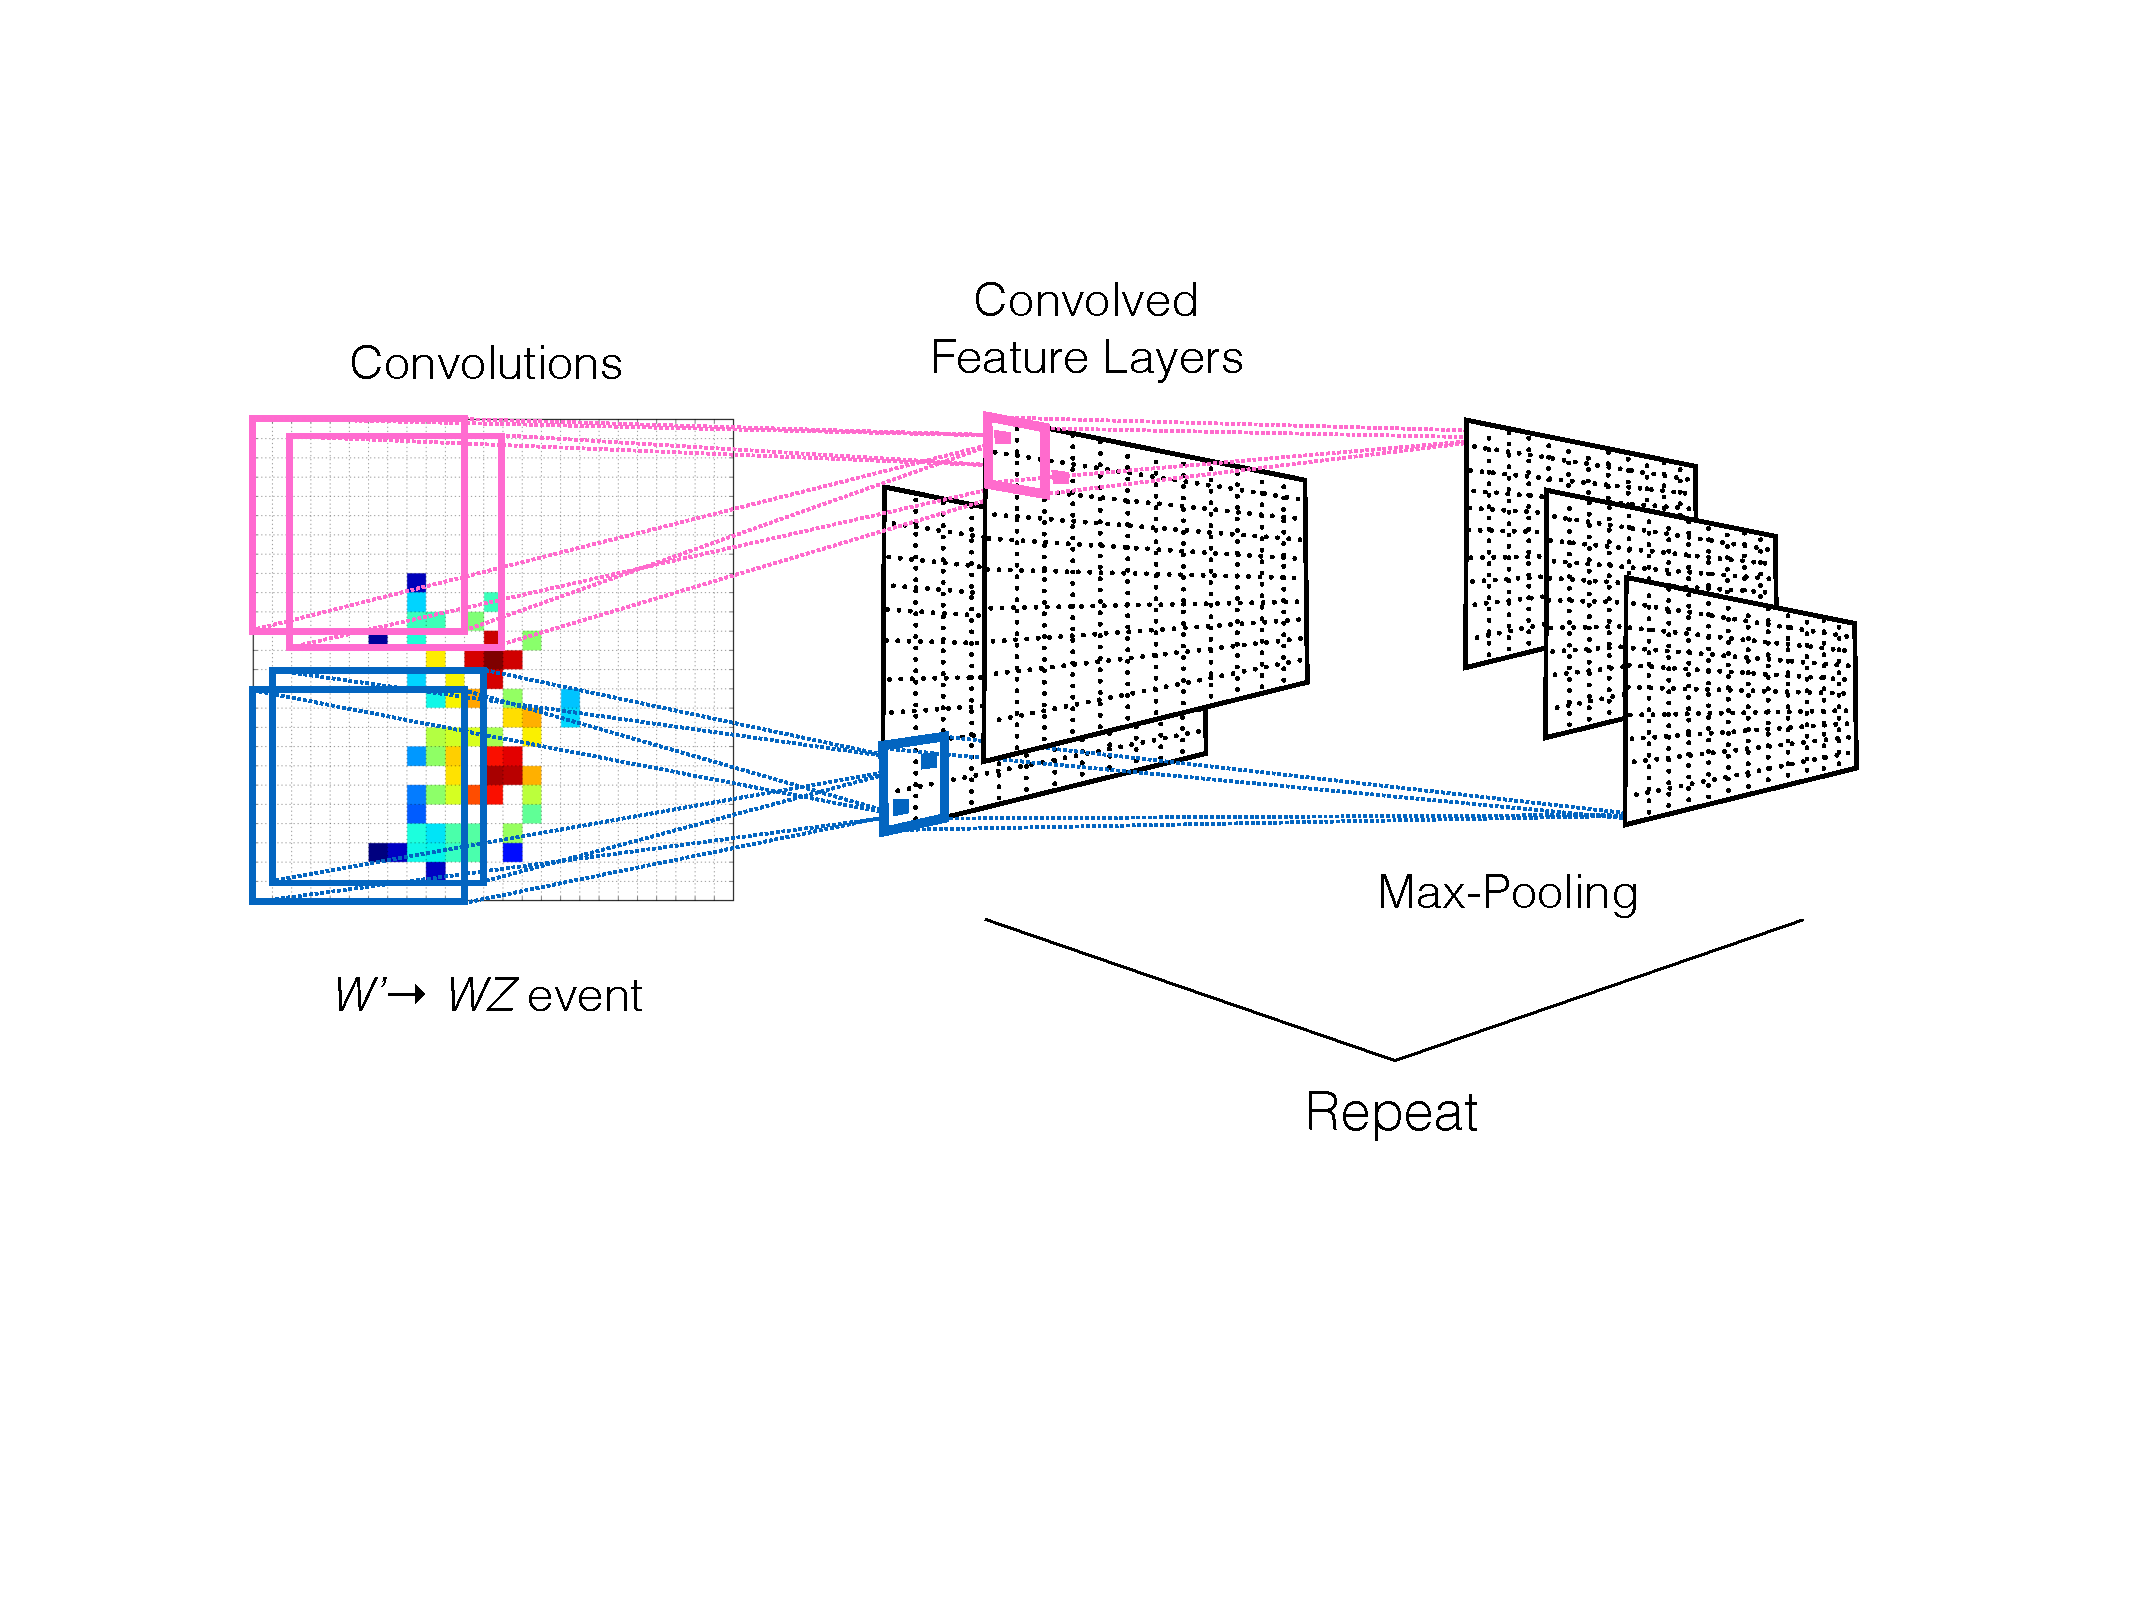
\includegraphics[width=0.75\textwidth]{figures/architecture.pdf}
  \caption{The convolution neural network concept as applied to jet-images.}
  \label{fig:arch}
\end{figure}

Our architecture can be succinctly written as 
\begin{equation}
  \mathtt{[Dropout \rightarrow Conv \rightarrow ReLU \rightarrow MaxPool] * 2 \rightarrow [Dropout \rightarrow FC \rightarrow ReLU] * 2 \rightarrow Sigmoid}.
\end{equation}

After early experiments with the standard $3\times 3$ kernel size, we discovered significantly worse performance over a more basic MaxOut \cite{maxout:goodfellow} feedforward network. After further investigation into larger convolutional kernel size, we discovered that larger-than-normal kernels work well on our application. Though not common in the Deep Learning community, we hypothesize that this larger kernel size is helpful when dealing with sparse structures in the input images. In Table~\ref{tab:kernelsize}, we show the optimal kernel size of $11\times11$ while considering the metric outlined in Section~\ref{sec:studies}.

\begin{table}[h!]
  \centering
  \begin{tabular}{r|c}
    \bfseries Kernel size & \bfseries AUC \\ 
    \hline
    $(3 \times 3)$ Conv & 14.770 \\
    \hline
    $(4 \times 4)$ Conv & 12.452 \\
    \hline
    $(5 \times 5)$ Conv & 11.061 \\
    \hline
    $(7 \times 7)$ Conv & 13.308 \\
    \hline
    $(9 \times 9)$ Conv & 17.291 \\
    \hline
    $(11 \times 11)$ Conv & 20.286 \\
    \hline
    $(15 \times 15)$ Conv & 18.140 \\
  \end{tabular}
  \caption{First layer convolution size vs. performance}
  \label{tab:kernelsize}
\end{table}
% table

We follow up the first layer of convolutions with Rectified Linear Unit activations, then utilize $(2, 2)$ max-pooling to downsample. We then use $(4\times 4)$ convolutions in the second convolutional unit + $(2, 2)$ max-pooling, and connect to 64 units then one final output.

Two convolution networks, which differ in their pre-processing, are studied in this paper.  The first, which we refer to as the ConvNet, is trained (and evaluated) on un-normalized jet-images using the transverse energy for the pixel intensities.  The second, which we refer to as ConvNet-Norm, is trained (and evaluated) on $L^{2}$ normalized jet-images using the energy for the pixel intensities.  Examining the performance of both networks allows us to study the possible effects of the pre-processing.



% subsubsection architectural_selection (end)

\subsubsection{Implementation and Training} % (fold)
\label{ssub:implementation_and_training}

Event generation and simulation was conducted on the SLAC \texttt{atlint} cluster. All Deep Learning experiments were conducted in Python with the Keras~\cite{Keras} Deep Learning library on the Stanford Institute for Computational and Mathematical Engineering GPU cluster, utilizing NVIDIA C2070 graphics cards. 

We used 30 million training and 30 million testing samples, and trained networks using both the Adam~\cite{DBLP:journals/corr/KingmaB14} algorithm and Stochastic Gradient Descent with Nesterov Momentum~\cite{Nesterov:1983wy}. We found that SGD+Nesterov outperformed Adam, and thus is used in all following facts and figures.

% subsubsection implementation_and_training (end)

